
\texttt{FastFEM} uses \texttt{PyVista}'s plotting capabilities for visual representation. There are currently six methods available to the user:

\begin{itemize}
    \item \texttt{define\_plotter()}: This is a helper method, responsible for interfacing the mesh object as produced by the mesher to \texttt{PyVista}'s own requirements. Notably, it returns a PyVista grid object containing all relevant information on the nodes and connectivity of the mesh, and is subsequently used for plotter generation.
    \item \texttt{plot\_mesh()}: This method is responsible for plotting the mesh object, and confirming \texttt{PyVista}'s redering is correct. In addition, it has aethetics related parameters that can be switched to the user's liking.
    \item \texttt{plot\_data()}: This method will plot the data on a mesh, without any time dependency. It is intended to either plot a single frame of the equation \ref{pde}, of its steady-state solution.
    \item \texttt{animate\_data()}: This method will plot the time-dependent data in an interactive window, such that the user can directly test the quality of their mesh/validity of their data.
    \item \texttt{make\_movie()}: This method will output a .mp4 file of the time-dependent data.
    \item \texttt{make\_gif()}: This method will output a .gif file of the time-dependent data.
\end{itemize}

Of most notable note, the interactive widnow generated by \texttt{plot\_mesh()} will strongly resemble the output as shown in figure \ref{fig:mesh}, but with higher customizability. A sample output is given in figure \ref{fig:PyVistaMesh}.

\begin{figure}[H]
    \centering
    \hfill
    \begin{subfigure}[c]{0.3\textwidth}
        \centering
        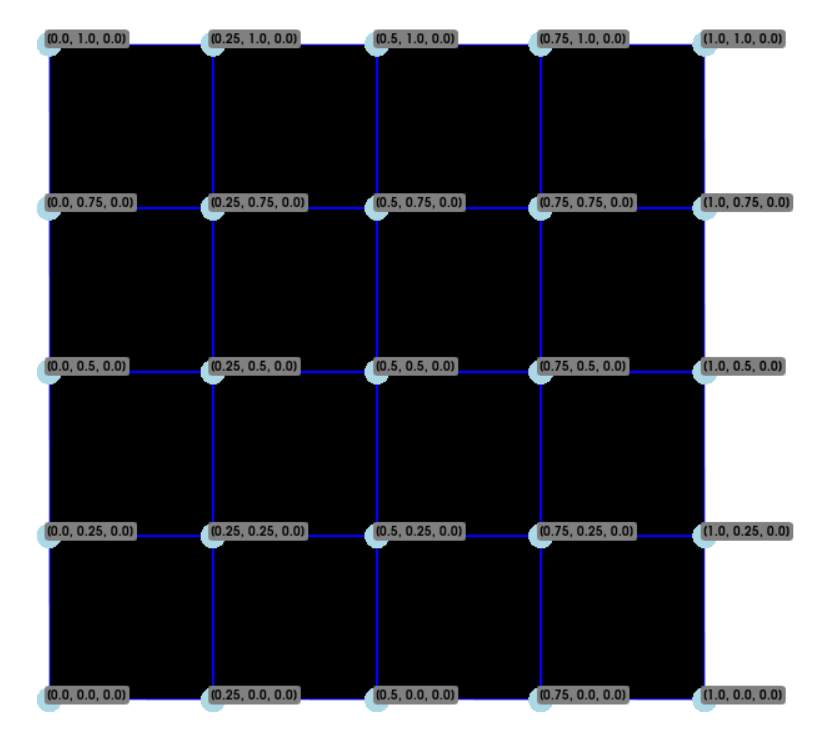
\includegraphics[width=\textwidth]{figures/PyVistaMesh_Customized.png}
        \caption{Ordered mesh, with quadrangles.}
        \label{fig:PyVistaMesh1}
    \end{subfigure}
    \hspace{0.1\textwidth}
    \begin{subfigure}[c]{0.4\textwidth}
        \centering
        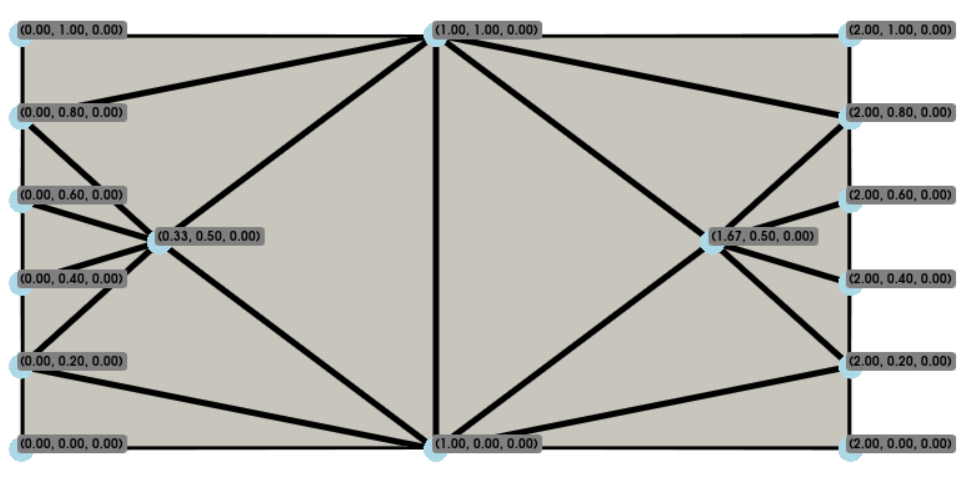
\includegraphics[width=\textwidth]{figures/PyVistaMesh_Customized2.png}
        \caption{Disordered mesh, with triangles.}
        \label{fig:PyVistaMesh2}
    \end{subfigure}
    \caption{Mesh outputs of \texttt{plot\_mesh()}, using \texttt{PyVista}'s rendering capabilities.}
    \label{fig:PyVistaMesh}
    \hfill
\end{figure}

Where the user may also interact with the mesh, and rotate it to any angle.

In addition, a single frame may also be plotted using the \texttt{plot\_data()} method, given the PDE has already been solved separately, and the content of each node in stored in a 3-dimensional array, for each time-step of the simulation. A sample output is given in figure \ref{fig:PyVistaPlotFrame}.

\begin{figure}[H]
    \centering
    \hfill
    \begin{subfigure}[c]{0.4\textwidth}
        \centering
        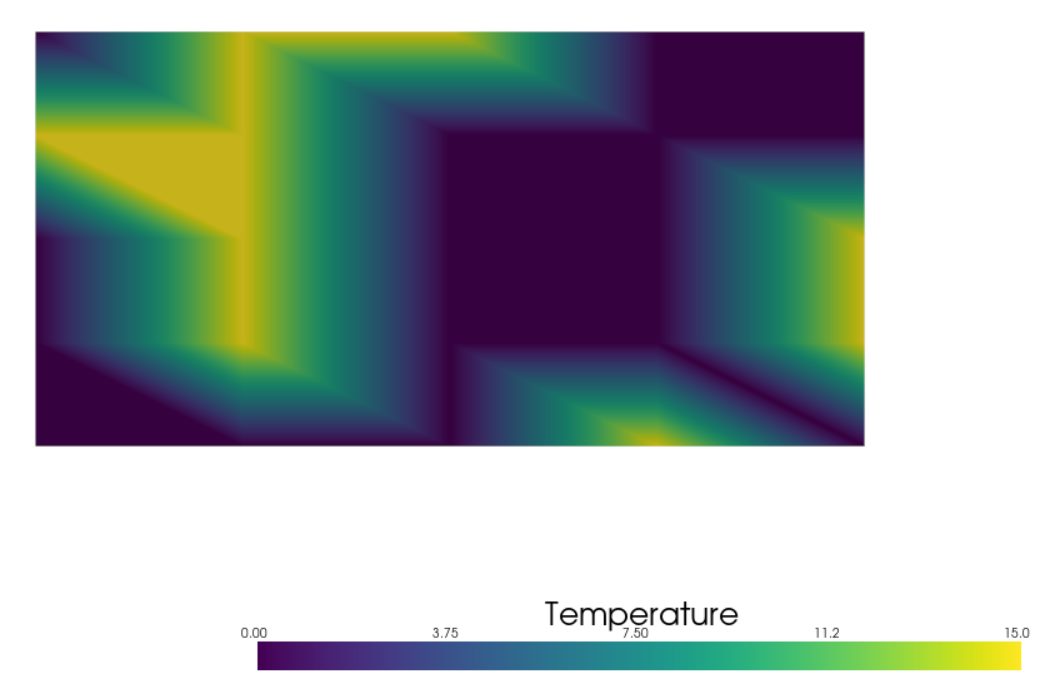
\includegraphics[width=\textwidth]{figures/PyVistaMesh_32.png}
        \caption{Plotted sample data, with 32 elements.}
        \label{fig:PyVistaMesh1}
    \end{subfigure}
    \hspace{0.1\textwidth}
    \begin{subfigure}[c]{0.4\textwidth}
        \centering
        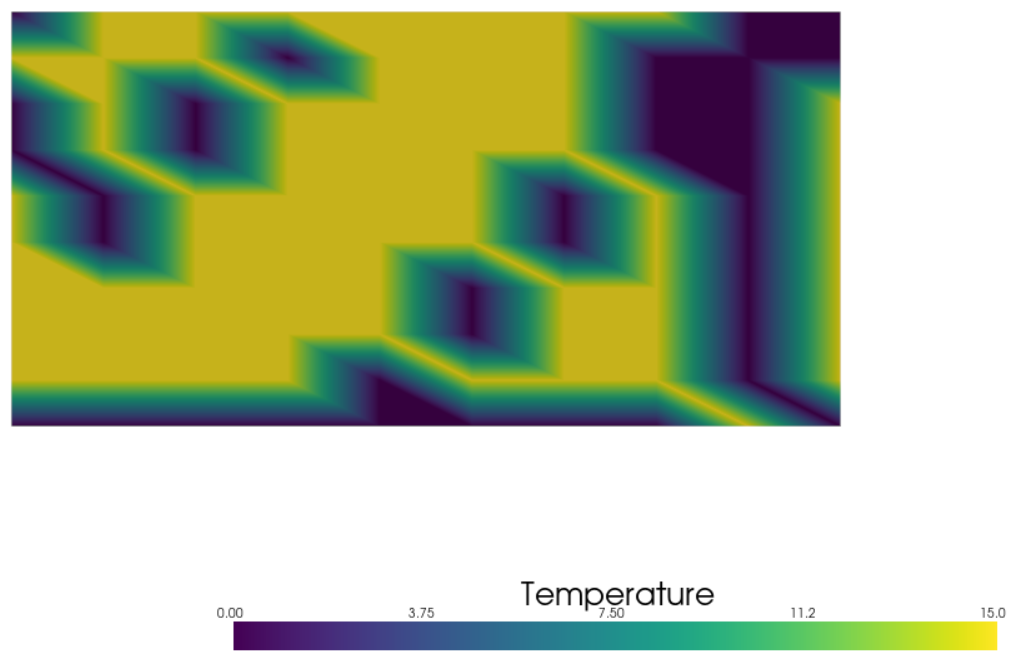
\includegraphics[width=\textwidth]{figures/PyVistaMesh_162.png}
        \caption{Plotted sample data, with 162 elements.}
        \label{fig:PyVistaMesh2}
    \end{subfigure}
    \caption{Outputs of \texttt{plot\_data()}.}
    \label{fig:PyVistaPlotFrame}
    \hfill
\end{figure}

Where the change in the number of elements accurately represents an increase in the resolution and quality of the solution.

In addition, another capability added by the \texttt{plotter} branch is the ability to animate the data interactively, and subsequently save a movie or gif of such data. A sample output is given in figure \ref{fig:PyVistaAnimated}.

\begin{figure}[H]
    \centering
    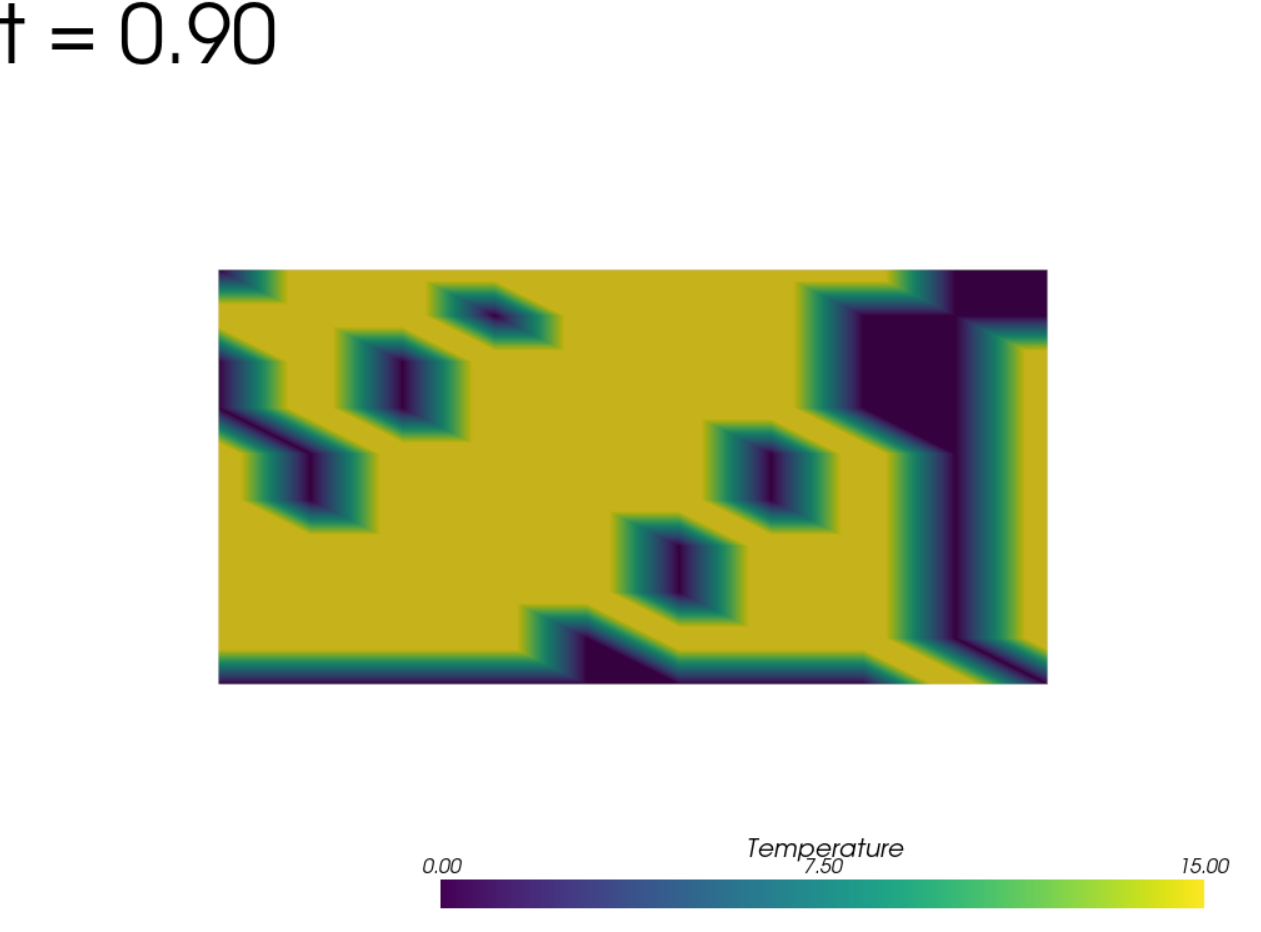
\includegraphics[width=0.5\textwidth]{figures/PyVista_Animated.png}
    \caption{A single frame of the animated data.}
    \label{fig:PyVistaAnimated}
\end{figure}

Where the most notable difference with the \texttt{plot\_data()} method is the plotted time at the top-left corner of the figure. In addition, using the \texttt{animate\_data()} method, the user has control over the number of frames per second of the animation, and enhance readability of the solution.

\textbf{Note}: Throughout the development of the \texttt{plotter} branch, testing remained a difficult aspect of the project. Many of the methods use rely on visual cues and generated plots to understand their validity. As such, the evaluation of the methods relied primarily in the assertion of the \textit{creation} of the method, rather than its actual content. To achieve this, \texttt{PyVista}'s show method (responsible for actually outputting the plot) was mocked using \texttt{unittest} and the \texttt{MonkeyPatch} testing fixture, such that no plot was actually generated thorugh the tests.

Another particular difficulty lied in the testing of the \texttt{make\_movie()} and \texttt{make\_gif()} methods, due to incompabilities of file writing across different operating systems and their reliance on external libraries, which resulted in tests passing locally but not through GitHub's CI pipeline. As such, these tests are currently skipped, while the issue is being actively debugged.
